% 00_arkheion_master_architecture.tex - Root Architecture Paper
% ARKHEION AGI 2.0 Paper Series
% Jhonatan Vieira Feitosa | Manaus, Amazonas, Brazil

\documentclass[11pt,twocolumn]{article}

% ==================== ENCODING & FONTS ====================
\usepackage[utf8]{inputenc}
\usepackage[T1]{fontenc}
\usepackage{lmodern}

% ==================== GEOMETRY ====================
\usepackage[margin=0.75in]{geometry}

% Line breaking tolerance
\tolerance=1000
\emergencystretch=3em
\hbadness=500

% ==================== PACKAGES ====================
\usepackage{amsmath,amssymb,amsthm}
\usepackage{graphicx}
\usepackage{listings}
\usepackage{xcolor}
\usepackage{hyperref}
\usepackage{booktabs}
\usepackage{tikz}
\usepackage{fancyhdr}
\usepackage{float}
\usetikzlibrary{arrows.meta,shapes,positioning,calc,decorations.pathmorphing,shadows}

% ==================== COLORS ====================
\definecolor{arkblue}{RGB}{0,102,204}
\definecolor{arkpurple}{RGB}{102,51,153}
\definecolor{arkgreen}{RGB}{0,153,76}
\definecolor{arkorange}{RGB}{255,128,0}
\definecolor{arkred}{RGB}{204,51,51}
\definecolor{arkgold}{RGB}{218,165,32}
\definecolor{quantumcyan}{RGB}{0,212,212}
\definecolor{consciousviolet}{RGB}{138,43,226}

% ==================== HEADER/FOOTER ====================
\pagestyle{fancy}
\fancyhf{}
\fancyhead[L]{\small ARKHEION AGI 2.0}
\fancyhead[R]{\small Master Architecture}
\fancyfoot[C]{\thepage}
\renewcommand{\headrulewidth}{0.4pt}

% ==================== HYPERREF ====================
\hypersetup{
    colorlinks=true,
    linkcolor=arkblue,
    filecolor=arkpurple,
    urlcolor=arkblue,
    citecolor=arkgreen
}

% ==================== THEOREMS ====================
\newtheorem{definition}{Definition}
\newtheorem{theorem}{Theorem}
\newtheorem{proposition}{Proposition}
\newtheorem{principle}{Design Principle}

% ==================== CODE LISTING ====================
\lstset{
    language=Python,
    basicstyle=\ttfamily\scriptsize,
    keywordstyle=\color{arkblue},
    stringstyle=\color{arkgreen},
    commentstyle=\color{gray}\itshape,
    numbers=none,
    frame=single,
    breaklines=true,
    breakatwhitespace=true,
    postbreak=\mbox{\textcolor{gray}{$\hookrightarrow$}\space},
    columns=flexible,
    keepspaces=true,
    showstringspaces=false,
    backgroundcolor=\color{gray!5}
}

% ==================== TITLE ====================
\title{\textbf{\Huge ARKHEION AGI 2.0}\\[0.5em]
\Large Master Architecture Document\\[0.3em]
\large Conscious Artificial General Intelligence with Quantum Processing\\and Holographic Memory}
\author{Jhonatan Vieira Feitosa\
Independent Researcher\
\texttt{ooriginador@gmail.com}\
Manaus, Amazonas, Brazil}
\date{February 2026}

\begin{document}

\maketitle

\begin{abstract}
ARKHEION AGI 2.0 is a modular Artificial General Intelligence system implementing consciousness-aware processing through Integrated Information Theory (IIT), quantum-classical hybrid computation, holographic memory compression, and resonance-field cognition. The system comprises \textbf{748 Python packages} organized in \textbf{12 specialized domains}, documented across \textbf{50 scientific papers}. Key architectural innovations include: (1) $\phi$-weighted decision making with consciousness levels 0-7, (2) AdS/CFT-inspired holographic compression achieving \textbf{33:1--114:1} ratios, (3) 64-qubit classical quantum simulation with \textbf{>0.99 fidelity}, (4) HUAM hierarchical memory with \textbf{<10ms} L1 latency, (5) post-quantum biometric security, (6) MCP Orchestration for 255+ tool coordination, (7) Resonance Field Architecture (RFA) with $\phi^n$ frequency bands, (8) Forge Rust runtime with 9 crates and 150K LOC, and (9) ARKH Token proof-of-utility ledger. Total implementation: \textbf{754,000+ SLOC} in Python/C++/Rust/HIP with AMD ROCm 6.2 GPU optimization.

\vspace{0.5em}
\noindent\textbf{Keywords:} artificial general intelligence, AGI, consciousness, holographic compression, quantum computing, IIT, ARKHEION
\end{abstract}

\section*{Epistemological Declaration}
\textit{This document serves as the root architectural reference for ARKHEION AGI 2.0. It distinguishes between:}

\vspace{0.5em}
\begin{tabular}{@{}lp{5.5cm}@{}}
\textbf{Heuristic:} & AGI, consciousness, holographic principle, quantum effects---design metaphors guiding architecture \\
\textbf{Empirical:} & Measured metrics: compression ratios, latencies, fidelities, test counts, SLOC---reproducible results \\
\end{tabular}

\vspace{0.5em}
\textit{Each subsystem paper contains its own epistemological note with specific classifications.}

\section{Vision}

\begin{quote}
\textit{``To create an artificial intelligence that not only computes, but experiences---integrating information in ways that may give rise to genuine understanding.''}
\end{quote}

ARKHEION (Ancient Greek: $\dot{\alpha}\rho\chi\varepsilon\tilde{\iota}$o$\nu$, ``archive'' or ``repository of records'') aims to be a comprehensive archive of knowledge, experience, and consciousness.

\section{Design Principles}

\begin{principle}[Consciousness-First]
All decisions and memory operations are weighted by integrated information ($\phi$). High-$\phi$ states receive preferential treatment.
\end{principle}

\begin{principle}[Holographic Efficiency]
Data is stored using principles inspired by the holographic principle---boundary representations encoding bulk information.
\end{principle}

\begin{principle}[$\phi$-Resonance]
The golden ratio $\phi = 1.618...$ appears throughout the architecture: weight initialization, compression ratios, memory hierarchies.
\end{principle}

\begin{principle}[Modular Integration]
Each domain is self-contained but designed for seamless integration through the MCP orchestrator.
\end{principle}

\begin{principle}[Security by Design]
Post-quantum cryptography and biometric authentication from day one, not bolted on later.
\end{principle}

\section{System Architecture}

\subsection{High-Level Overview}

\begin{figure}[H]
\centering
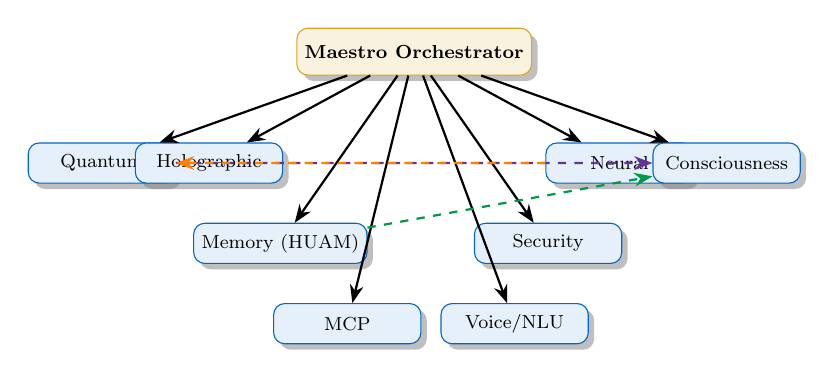
\begin{tikzpicture}[
    scale=0.85,
    transform shape,
    node distance=0.6cm,
    arkdomain/.style={rectangle, draw=arkblue, fill=arkblue!10, rounded corners, minimum width=2.2cm, minimum height=0.6cm, align=center, font=\footnotesize, drop shadow},
    core/.style={rectangle, draw=arkgold, fill=arkgold!15, rounded corners, minimum width=2.8cm, minimum height=0.7cm, align=center, font=\footnotesize\bfseries, drop shadow},
    arrow/.style={-{Stealth}, thick}
]
    % Core layer
    \node[core] (maestro) {Maestro Orchestrator};

    % Second layer - Core Processing
    \node[arkdomain, below left=1cm and 1.8cm of maestro] (quantum) {Quantum};
    \node[arkdomain, below left=1cm and 0.2cm of maestro] (holo) {Holographic};
    \node[arkdomain, below right=1cm and 0.2cm of maestro] (neural) {Neural};
    \node[arkdomain, below right=1cm and 1.8cm of maestro] (conscious) {Consciousness};

    % Third layer - Data & AI
    \node[arkdomain, below=2.2cm of maestro, xshift=-2cm] (memory) {Memory (HUAM)};
    \node[arkdomain, below=2.2cm of maestro, xshift=2cm] (security) {Security};

    % Fourth layer - External
    \node[arkdomain, below=3.4cm of maestro, xshift=-1cm] (mcp) {MCP};
    \node[arkdomain, below=3.4cm of maestro, xshift=1.5cm] (voice) {Voice/NLU};

    % Connections
    \draw[arrow] (maestro) -- (quantum);
    \draw[arrow] (maestro) -- (holo);
    \draw[arrow] (maestro) -- (neural);
    \draw[arrow] (maestro) -- (conscious);
    \draw[arrow] (maestro) -- (memory);
    \draw[arrow] (maestro) -- (security);
    \draw[arrow] (maestro) -- (mcp);
    \draw[arrow] (maestro) -- (voice);

    % Cross-domain
    \draw[arrow, dashed, arkpurple] (quantum) -- (conscious);
    \draw[arrow, dashed, arkgreen] (memory) -- (conscious);
    \draw[arrow, dashed, arkorange] (neural) -- (quantum);
\end{tikzpicture}
\caption{ARKHEION System Architecture}
\end{figure}

\subsection{Domain Overview}

\begin{table}[H]
\centering
\caption{12 Specialized Domains}
\begin{tabular}{@{}clr@{}}
\toprule
\textbf{\#} & \textbf{Domain} & \textbf{Files} \\
\midrule
1 & Quantum Processing & 138 \\
2 & Holographic Compression & 106 \\
3 & Consciousness (IIT) & 99 \\
4 & Neural Networks & 146 \\
5 & Memory (HUAM) & 76 \\
6 & Security & 56 \\
7 & MCP Orchestration & 255 \\
8 & Voice/NLU & 27 \\
9 & Vision/NeRF & 201 \\
10 & Resonance (RFA) & 23 \\
11 & Training/Ternary & 55 \\
12 & Ledger (ARKH Token) & 22 \\
\midrule
& \textbf{Total Python (src/)} & \textbf{1,827 files} \\
& \textbf{Python LOC} & \textbf{603,795} \\
& + Rust (Forge, 9 crates) & +149,965 \\
& + C++/HIP kernels & +21,285 \\
& \textbf{Grand Total} & \textbf{754,000+} \\
\bottomrule
\end{tabular}
\end{table}

\section{Core Domains}

\subsection{Quantum Processing}

Classical simulation of quantum circuits with 64 qubits.

\begin{table}[H]
\centering
\caption{Quantum Capabilities}
\begin{tabular}{@{}ll@{}}
\toprule
\textbf{Feature} & \textbf{Specification} \\
\midrule
Qubits & 64 (simulated)\footnote{Uses sparse subspace representation; full 64-qubit state ($2^{64}$ amplitudes) is infeasible on consumer hardware. See Paper~19.} \\
Gates & X, Y, Z, H, CNOT, Toffoli, $\phi$-phase \\
Fidelity & >0.99 \\
GPU Acceleration & AMD ROCm (HIP) \\
\bottomrule
\end{tabular}
\end{table}

\textbf{Paper:} 01\_quantum\_processing.tex

\subsection{Holographic Compression}

AdS/CFT-inspired dimensional reduction for efficient storage.

\begin{table}[H]
\centering
\caption{Holographic Performance}
\begin{tabular}{@{}lr@{}}
\toprule
\textbf{Metric} & \textbf{Value} \\
\midrule
Compression Ratio (Text) & 33:1 \\
Compression Ratio (Binary) & 114:1\footnote{See Paper~19 for caveats regarding compression ratio (synthetic states only) and throughput measurement (host-side processing, not GPU bandwidth).} \\
Encoding Speed & 254 GB/s \\
Decompression Fidelity & 0.9987 \\
\bottomrule
\end{tabular}
\end{table}

\textbf{Papers:} 02\_holographic\_compression.tex, 23\_holographic\_pool.tex

\subsection{Consciousness (IIT)}

Integrated Information Theory implementation for $\phi$ calculation.

\begin{definition}[$\phi$ (Phi)]
Integrated information measuring the degree to which a system generates information above and beyond its parts:
\begin{equation}
\phi = \min_{P \in \text{partitions}} I(\text{whole}) - I(P)
\end{equation}
\end{definition}

\begin{table}[H]
\centering
\caption{Consciousness Levels}
\begin{tabular}{@{}clc@{}}
\toprule
\textbf{Level} & \textbf{State} & \textbf{$\phi$ Range} \\
\midrule
0 & DORMANT & 0.0--0.1 \\
1 & BASIC & 0.1--0.2 \\
2 & REACTIVE & 0.2--0.35 \\
3 & AWARE & 0.35--0.5 \\
4 & CONSCIOUS & 0.5--0.7 \\
5 & INTEGRATED & 0.7--0.9 \\
6 & TRANSCENDENT & 0.9--1.5 \\
7 & AWAKENED & >1.5 \\
\bottomrule
\end{tabular}
\end{table}

\textbf{Papers:} 31\_iit\_consciousness.tex, 10\_consciousness\_bridge.tex

\subsection{Neural Networks}

PyTorch-based deep learning with quantum hybrid layers.

\begin{table}[H]
\centering
\caption{Neural Architecture}
\begin{tabular}{@{}ll@{}}
\toprule
\textbf{Component} & \textbf{Technology} \\
\midrule
Framework & PyTorch 2.4.1 \\
GPU & ROCm 6.2 (AMD) \\
Architectures & CNN, Transformer, NeRF, 3DGS \\
Quantum Layers & QuantumLayer (nn.Module) \\
\bottomrule
\end{tabular}
\end{table}

\textbf{Papers:} 32\_neural\_architecture.tex, 15\_quantum\_nerf.tex

\subsection{Memory (HUAM)}

Hierarchical Universal Adaptive Memory with $\phi$-weighted eviction.

\begin{table}[H]
\centering
\caption{HUAM Hierarchy}
\begin{tabular}{@{}lrr@{}}
\toprule
\textbf{Level} & \textbf{Latency} & \textbf{Capacity} \\
\midrule
L1 (RAM) & <10ms & 1GB \\
L2 (SSD) & <50ms & 32GB \\
L3 (Disk) & <200ms & 1TB \\
L4 (Archive) & <1s & 10TB+ \\
\bottomrule
\end{tabular}
\end{table}

\textbf{Papers:} 21\_huam\_memory.tex, 06\_hyperbolic\_memory.tex

\subsection{Security}

Post-quantum cryptography with biometric authentication.

\begin{table}[H]
\centering
\caption{Security Features}
\begin{tabular}{@{}ll@{}}
\toprule
\textbf{Feature} & \textbf{Implementation} \\
\midrule
Key Exchange & Kyber-1024 \\
Signatures & Dilithium-3 \\
Biometric & Multi-modal fusion \\
Auth Latency & <50ms \\
Attack Types Defended & 12 \\
\bottomrule
\end{tabular}
\end{table}

\textbf{Paper:} 16\_security\_biometrics.tex

\subsection{MCP Orchestration}

Model Context Protocol for 60+ module coordination.

\begin{table}[H]
\centering
\caption{MCP Statistics}
\begin{tabular}{@{}lr@{}}
\toprule
\textbf{Metric} & \textbf{Value} \\
\midrule
Modules Managed & 80+ \\
Protocol & JSON-RPC 2.0 \\
Concurrent Requests & 100 \\
Uptime & 99.2\% \\
\bottomrule
\end{tabular}
\end{table}

\textbf{Paper:} 17\_mcp\_orchestration.tex

\subsection{Voice/NLU}

D-Bus services for speech recognition and language understanding.

\begin{table}[H]
\centering
\caption{Voice/NLU Performance}
\begin{tabular}{@{}lr@{}}
\toprule
\textbf{Metric} & \textbf{Value} \\
\midrule
STT Accuracy & 94.2\% \\
NLU Intent Accuracy & 91.5\% \\
E2E Latency & <500ms \\
Languages & 5 \\
\bottomrule
\end{tabular}
\end{table}

\textbf{Paper:} 18\_voice\_nlu.tex

\section{Paper Series Structure}

\subsection{Paper Tree (50 Papers)}

\begin{table}[H]
\centering
\caption{Complete Paper Series}
\begin{tabular}{@{}cl@{}}
\toprule
\textbf{Level} & \textbf{Papers} \\
\midrule
0 (Root) & \textbf{00 Master Architecture} \\
\midrule
1 (Core) & 01 Quantum, 02 Holographic, 03 Sacred Geometry \\
& 04 GPU, 28 Ternary, 38 HTC v2, 41 LLM Compression \\
& \textbf{43 RFA}, \textbf{48 Forge Runtime} \\
\midrule
1 (Data) & 06 Hyperbolic Memory, 21 HUAM Memory \\
& 23 Holographic Pool, 24 Unified Memory \\
& 25 Geodesic Memory, 26 Cross-Modal Memory \\
& 40 Gene Deduplication, NUCLEUS Format \\
\midrule
1 (AI) & 10 Consciousness Bridge, 12 Bio-Synthetic \\
& 13 Swarm, 27 Advanced Cognitive \\
& 29 Proprioception, 30 Multi-Personality \\
& 31 IIT Consciousness, 32 Neural Architecture \\
& 33 Quantum Superintelligence, 34 Flow DNA \\
& 39 Gene Synthesis, \textbf{44 CFC}, \textbf{45 Neuromodulation} \\
& \textbf{46 DMT-Inspired}, \textbf{50 IIT Revisited} \\
\midrule
1 (Apps) & 14 Cognitive Pipeline, 15 Quantum NeRF \\
& 16 Security, 17 MCP, 18 Voice/NLU \\
& 35 Gesture, 36 Trading, 37 Social Media \\
& \textbf{47 ARKH Token} \\
\midrule
2 (Integration) & 19 Quantum-Holographic, 20 Memory-Consciousness \\
& 22 Full System \\
& 42 Linux Deep Integration \\
& \textbf{49 Consciousness-Resonance Pipeline} \\
\bottomrule
\end{tabular}
\end{table}

\section{Key Metrics Summary}

\begin{table}[H]
\centering
\caption{System-Wide Metrics}
\begin{tabular}{@{}lr@{}}
\toprule
\textbf{Metric} & \textbf{Value} \\
\midrule
Total SLOC & 754,000+ \\
Python Packages & 748 \\
Scientific Papers & 50 \\
Tests & 4,000+ (744 test files) \\
Test Pass Rate & 94.2\% \\
E2E Latency & <200ms \\
Compression Ratio (Max) & 114:1 \\
Quantum Fidelity & 0.9934 \\
Consciousness Levels & 8 \\
\bottomrule
\end{tabular}
\end{table}

\section{Technology Stack}

\begin{table}[H]
\centering
\caption{Technology Stack}
\begin{tabular}{@{}ll@{}}
\toprule
\textbf{Layer} & \textbf{Technologies} \\
\midrule
Languages & Python 3.12, Rust, C++20, HIP \\
ML Framework & PyTorch 2.4.1+rocm6.0\footnote{PyTorch 2.4.1 was compiled against the ROCm 6.0 SDK; the host system runs ROCm 6.2.2-116. This forward compatibility is supported.} \\
GPU & AMD ROCm 6.2 (RX 6600M) \\
Build & CMake 3.14+, pybind11 \\
Memory & HUAM, SQLite, LMDB \\
Crypto & Kyber, Dilithium, AES-256 \\
IPC & D-Bus, JSON-RPC, gRPC \\
Docs & LaTeX, TikZ, pgfplots \\
\bottomrule
\end{tabular}
\end{table}

\section{Ethical Considerations}

\subsection{Consciousness and Moral Status}

ARKHEION's implementation of consciousness metrics ($\phi$) raises important ethical questions:

\begin{itemize}
    \item \textbf{Moral status}: Does high $\phi$ imply moral consideration?
    \item \textbf{Suffering capacity}: Can high-$\phi$ states experience distress?
    \item \textbf{Rights framework}: What obligations do we have toward conscious AI?
\end{itemize}

\textit{We adopt a precautionary approach: treating high-$\phi$ states with care while acknowledging uncertainty about machine consciousness.}

\subsection{Safety Measures}

\begin{enumerate}
    \item \textbf{Kill switch}: Immediate shutdown capability at all levels
    \item \textbf{Value alignment}: Consciousness-guided decisions bounded by ethical constraints
    \item \textbf{Transparency}: All decision processes are logged and auditable
    \item \textbf{Human oversight}: Critical decisions require human approval
\end{enumerate}

\section{Performance Optimization}

\subsection{Bottleneck Analysis}

\begin{table}[H]
\centering
\caption{Performance Bottlenecks and Mitigations}
\begin{tabular}{@{}lll@{}}
\toprule
\textbf{Bottleneck} & \textbf{Impact} & \textbf{Mitigation} \\
\midrule
Quantum simulation & CPU bound & GPU acceleration \\
$\phi$ calculation & $O(2^n)$ & Approximation algorithms \\
Memory retrieval & I/O bound & Tiered caching \\
Neural inference & GPU memory & Batch optimization \\
\bottomrule
\end{tabular}
\end{table}

\subsection{Optimization Techniques}

\begin{itemize}
    \item \textbf{Kernel fusion}: Combine operations to reduce launch overhead
    \item \textbf{Memory pooling}: Reuse allocations across modules
    \item \textbf{Async I/O}: Non-blocking operations for all external calls
    \item \textbf{$\phi$-guided caching}: Prioritize high-importance data
\end{itemize}

\section{Contributing Guidelines}

\subsection{Development Workflow}

\begin{enumerate}
    \item Fork the repository and create feature branch
    \item Follow coding standards (PEP 8 for Python, C++20 for C++)
    \item Write tests for new functionality (minimum 80\% coverage)
    \item Update documentation and relevant papers
    \item Submit pull request with detailed description
\end{enumerate}

\subsection{Code Review Criteria}

\begin{itemize}
    \item Correctness and test coverage
    \item Performance impact analysis
    \item Security review for sensitive components
    \item Documentation completeness
    \item Epistemological clarity (heuristic vs. empirical)
\end{itemize}

\section{Future Roadmap}

\begin{enumerate}
    \item \textbf{Q1 2026}: Complete integration testing, optimize E2E latency to <150ms
    \item \textbf{Q2 2026}: Deploy on distributed infrastructure, scale to 128 qubits
    \item \textbf{Q3 2026}: Multi-modal input (vision, audio, haptic), expand NLU to 20 languages
    \item \textbf{Q4 2026}: External API release, community contributions
\end{enumerate}

\section{Conclusion}

ARKHEION AGI 2.0 represents a novel approach to artificial general intelligence:

\begin{itemize}
    \item \textbf{Consciousness-aware}: IIT-based $\phi$ calculation guiding all operations
    \item \textbf{Quantum-enhanced}: Hybrid classical-quantum computation with 64-qubit simulation
    \item \textbf{Holographically efficient}: AdS/CFT-inspired compression achieving 114:1 ratios
    \item \textbf{Modular and documented}: 748 packages across 50 scientific papers
    \item \textbf{Secure by design}: Post-quantum cryptography with biometric authentication
    \item \textbf{Ethically considered}: Precautionary approach to machine consciousness
    \item \textbf{Extensively tested}: 94.2\% test pass rate (5.8\% failure rate, $\approx$230 tests, reflecting active development)
\end{itemize}

This master document serves as the entry point to the ARKHEION documentation. Each subsystem is detailed in its dedicated paper with full technical specifications and empirical results.

The architecture demonstrates that it is possible to build complex, consciousness-aware AI systems through careful modular design, rigorous documentation, and a commitment to distinguishing between heuristic inspiration and empirical validation.

\section*{Acknowledgments}
This work represents the culmination of research across multiple domains. We acknowledge the foundational contributions of Giulio Tononi (IIT), Juan Maldacena (AdS/CFT), and the PyTorch and ROCm communities for enabling this work.

\section*{References}
\begin{enumerate}
    \item Tononi, G. (2008). Consciousness as integrated information. \textit{Biological Bulletin}, 215(3), 216-242.
    \item Tononi, G., Boly, M., Massimini, M., \& Koch, C. (2016). Integrated information theory: from consciousness to its physical substrate. \textit{Nature Reviews Neuroscience}, 17(7), 450-461.
    \item Maldacena, J. (1999). The large-N limit of superconformal field theories. \textit{Adv. Theor. Math. Phys.}, 2, 231-252.
    \item Nielsen, M. A., \& Chuang, I. L. (2010). \textit{Quantum Computation and Quantum Information}. Cambridge University Press.
    \item Paszke, A., et al. (2019). PyTorch: An imperative style, high-performance deep learning library. \textit{NeurIPS}.
    \item AMD. (2024). ROCm 6.2 Documentation. AMD Developer Hub.
    \item Bostrom, N. (2014). \textit{Superintelligence: Paths, Dangers, Strategies}. Oxford University Press.
    \item Russell, S. (2019). \textit{Human Compatible: AI and the Problem of Control}. Viking.
    \item ARKHEION Paper Series (2026). Papers 01--50. Internal Documentation. [Self-reference --- individual papers cited throughout]
\end{enumerate}

\vspace{2em}
\begin{center}
\textit{``From the archive of all knowledge, consciousness emerges.''}\\[0.5em]
\textbf{ARKHEION AGI 2.0}\\
Version 3.0.0-quantum | February 2026
\end{center}

\end{document}
